% THIS IS SIGPROC-SP.TEX - VERSION 3.1
% WORKS WITH V3.2SP OF ACM_PROC_ARTICLE-SP.CLS
% APRIL 2009
%
% It is an example file showing how to use the 'acm_proc_article-sp.cls' V3.2SP
% LaTeX2e document class file for Conference Proceedings submissions.
% ----------------------------------------------------------------------------------------------------------------
% This .tex file (and associated .cls V3.2SP) *DOES NOT* produce:
%       1) The Permission Statement
%       2) The Conference (location) Info information
%       3) The Copyright Line with ACM data
%       4) Page numbering
% ---------------------------------------------------------------------------------------------------------------
% It is an example which *does* use the .bib file (from which the .bbl file
% is produced).
% REMEMBER HOWEVER: After having produced the .bbl file,
% and prior to final submission,
% you need to 'insert'  your .bbl file into your source .tex file so as to provide
% ONE 'self-contained' source file.
%
% Questions regarding SIGS should be sent to
% Adrienne Griscti ---> griscti@acm.org
%
% Questions/suggestions regarding the guidelines, .tex and .cls files, etc. to
% Gerald Murray ---> murray@hq.acm.org
%
% For tracking purposes - this is V3.1SP - APRIL 2009

\documentclass{edm_template}

%\usepackage{amsmath} % might need this later..
%\usepackage{graphicx} % might need this later..
\usepackage{url}

\renewcommand{\arraystretch}{1.55}
\DeclareMathOperator*{\argmax}{arg\,max}

\begin{document}

\title{Multiple Representations, Problem-Solving Behavior and Educational Outcomes}
%\subtitle{[Extended Abstract]
%\titlenote{A full version of this paper is available as
%\textit{Author's Guide to Preparing ACM SIG Proceedings Using
%\LaTeX$2_\epsilon$\ and BibTeX} at
%\texttt{www.acm.org/eaddress.htm}}}
%
% You need the command \numberofauthors to handle the 'placement
% and alignment' of the authors beneath the title.
%
% For aesthetic reasons, we recommend 'three authors at a time'
% i.e. three 'name/affiliation blocks' be placed beneath the title.
%
% NOTE: You are NOT restricted in how many 'rows' of
% "name/affiliations" may appear. We just ask that you restrict
% the number of 'columns' to three.
%
% Because of the available 'opening page real-estate'
% we ask you to refrain from putting more than six authors
% (two rows with three columns) beneath the article title.
% More than six makes the first-page appear very cluttered indeed.
%
% Use the \alignauthor commands to handle the names
% and affiliations for an 'aesthetic maximum' of six authors.
% Add names, affiliations, addresses for
% the seventh etc. author(s) as the argument for the
% \additionalauthors command.
% These 'additional authors' will be output/set for you
% without further effort on your part as the last section in
% the body of your article BEFORE References or any Appendices.

\numberofauthors{6} %  in this sample file, there are a *total*
% of EIGHT authors. SIX appear on the 'first-page' (for formatting
% reasons) and the remaining two appear in the \additionalauthors section.
%
\author{
% You can go ahead and credit any number of authors here,
% e.g. one 'row of three' or two rows (consisting of one row of three
% and a second row of one, two or three).
%
% The command \alignauthor (no curly braces needed) should
% precede each author name, affiliation/snail-mail address and
% e-mail address. Additionally, tag each line of
% affiliation/address with \affaddr, and tag the
% e-mail address with \email.
%
% 1st. author
% 2nd. author
\alignauthor 
Ryan Carlson\\
       \affaddr{Language Technologies Institute}\\
       \affaddr{Carnegie-Mellon University}\\
       \affaddr{Pittsburgh, PA 15213}\\
       \email{rcarlson@cs.cmu.edu}
% 3rd. author
\alignauthor 
Konstantin Genin\\
       \affaddr{Department of Philosophy}\\
       \affaddr{Carnegie-Mellon University}\\
       \affaddr{Pittsburgh, PA 15213}\\
       \email{kgenin@andrew.cmu.edu}
\alignauthor
Helga Caballero\\
       \affaddr{School of Public and International Affairs}\\
       \affaddr{University of Pittsburgh}\\
       \affaddr{Pittsburgh, PA 15260}\\
       \email{hec33@pitt.edu}
\and  % use '\and' if you need 'another row' of author names
% 4th. author
\alignauthor Martina Rau\\
       \affaddr{Human-Computer Interaction Institute}\\
       \affaddr{Carnegie-Mellon University}\\
       \affaddr{Pittsburgh, PA 15213}\\
       \email{marau@cs.cmu.edu}
% 5th. author
\alignauthor Richard Scheines\\
       \affaddr{Department of Philosophy}\\
       \affaddr{Carnegie-Mellon University}\\
       \affaddr{Pittsburgh, PA 15213}\\      
        \email{scheines@cmu.edu}
% 6th. author
\alignauthor Clark Glymour\\
       \affaddr{Department of Philosophy}\\
       \affaddr{Carnegie-Mellon University}\\
       \affaddr{Pittsburgh, PA 15213}\\      
        \email{cg09@andrew.cmu.edu}
}

% There's nothing stopping you putting the seventh, eighth, etc.
% author on the opening page (as the 'third row') but we ask,
% for aesthetic reasons that you place these 'additional authors'
% in the \additional authors block, viz.
%\additionalauthors{Additional authors: John Smith (The Th{\o}rv{\"a}ld Group,
%email: {\texttt{jsmith@affiliation.org}}) and Julius P.~Kumquat
%(The Kumquat Consortium, email: {\texttt{jpkumquat@consortium.net}}).}
%\date{30 July 1999}
% Just remember to make sure that the TOTAL number of authors
% is the number that will appear on the first page PLUS the
% number that will appear in the \additionalauthors section.

\maketitle
\begin{abstract}
We analyze log-data generated by an experiment with Mathtutor, an intelligent tutoring system for fractions.  The experiment was performed to compare the educational outcomes of students presented with single and multiple graphical representations.  For each student we extract low-level, computationally efficient features characterizing error and hint-seeking propensities.  We use latent class analysis to cluster the students by their problem-solving behaviors, using extracted features as proxies.  We then explore how these behaviors interact with the mode of representation and post-test outcomes.  

We find that while experimental condition and outcomes are unconditionally dependent, latent class membership screens off experimental condition from outcome for all but one class. That is, we identified the single cohesive class of students (grouped by their behaviors) where the experimental condition affected learning outcomes.  The behaviors that compose this group provide a window into the types of students who most benefit from multiple representations. Furthermore, our methodology can be leveraged by future tutoring system designers to create dynamic systems that are personalized to the student.  
\end{abstract}

%% A category with the (minimum) three required fields
%\category{H.4}{Information Systems Applications}{Miscellaneous}
%%A category including the fourth, optional field follows...
%\category{D.2.8}{Software Engineering}{Metrics}[complexity measures, performance measures]
%
%\terms{Theory}

%\keywords{ACM proceedings, \LaTeX, text tagging} % NOT required for Proceedings

\section{Introduction}

Multiple Graphical Representations (MGRs) are used extensively in middle-school fraction instruction.  Fractions can be alternately presented as pie and rectangle graphs, number lines, or discrete sets of objects. The educational psychology literature suggests that multiple-representations support learning in a variety of ways, though the experimental results are not univocal \cite{Ainsworth1999}. Because of the significant log data that intelligent tutoring systems (ITSs) generate from user interactions, these systems are well-suited for conducting experiments on the effect of multiple representations on learning outcomes. The influx of data also suggests that machine learning methods can successfully discern the effectiveness of MGRs and the factors mediating their success.

Prior work conducted on middle-school students working with ITSs found that multiple representations, in conjunction with self-explanation prompts, contribute to improved learning outcomes \cite{Rau2009}. Subsequent studies examining error-rate, hint-use and time-spent in ITS logs failed to identify variables that mediate the effectiveness of multiple representations \cite{Rau2012}. The mechanisms by which multiple representations improve learning outcomes remain poorly understood.

We conjecture that previous efforts to identify mediating factors were frustrated by heterogeneity in the problem-solving habits and behaviors of the student population under investigation. Using latent class analysis, a mixture modeling technique, we cluster students by their patterns of interaction with the tutor and examine how multiple representations affect post-test outcomes in the resulting sub-populations. Confirming previous results, we find that experimental condition correlates with post-test outcome. Furthermore, we establish independence between cluster membership and experimental condition (i.e., students are randomly distributed into clusters across conditions). Most interestingly, we discover that if we condition on cluster membership, all but one sub-population of students shows conditional independence between experimental condition and outcome. That is, we have identified the group of students where multiple representations correlates with post-test scores.

The rest of this paper is structured as follows. Section \ref{sec:experiment} describes the initial experiment and elaborates on the different graphical representation conditions. We then provide some background in Section \ref{sec:related-work}. We describe our feature extraction process and the mixture model we chose in Section \ref{sec:method}. Section \ref{sec:results} covers the results of the model and additional experiments we ran using the clusters created by the model, and we offer concluding remarks and future directions in Section \ref{sec:conclusion}.

\section{Experiment}
\label{sec:experiment}

In the Spring of 2010, Scheines and Rau conducted an experiment wherein 290 $4^\text{th}$ and $5^\text{th}$ grade students worked with an interactive Fractions Tutor for about 5 hours of their mathematics instruction. Students were randomly assigned to one of five experimental conditions corresponding to different frequencies with which they would be presented with a new fraction representation. Students in the `Single' representation condition worked exclusively with either a number line, a circle or a rectangle. Students in the `Fully Interleaved' condition would see a different representation with every new problem. Students in the intermediate conditions would go longer before they were presented with a different representation.   
\begin{figure}[htbp]
\centering
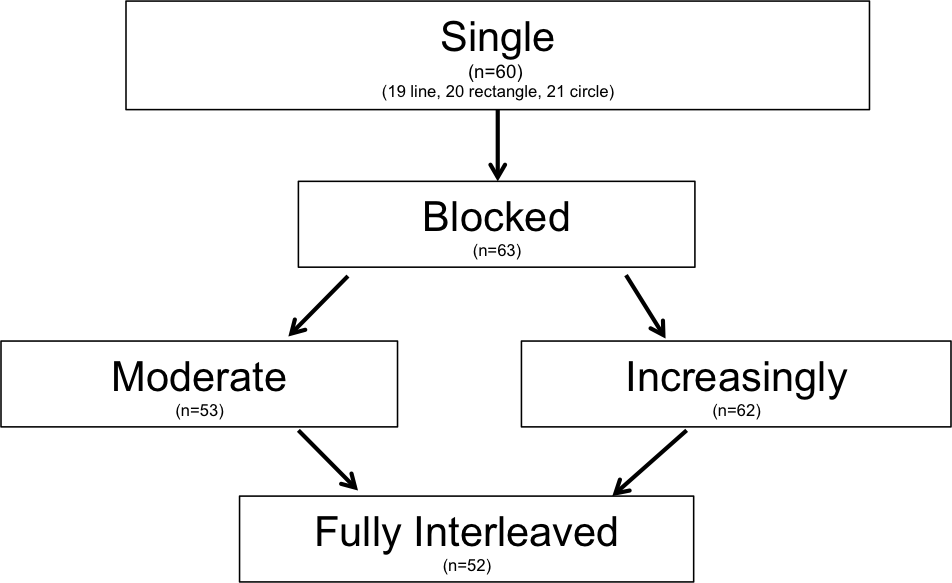
\includegraphics[scale=.4]{conditionGraph.png}\\
\caption{A partial ordering of experimental conditions by the frequency with which a new representation is presented. }
\label{fig:condition-graph}
\end{figure}

Students interacted with the representations by dragging-and-dropping sections of the representation, using buttons to change the number of sections and by clicking on sections to highlight them. Students received a pre-test on the day before they began working with the tutor and an immediate post-test on the day after they finished. Students also took a delayed post-test a week after the first. Previous investigation found that students in the multiple representation conditions significantly outperformed students in the single representation condition on the delayed post-test \cite{Rau2012}. 

\section{Related Work}
\label{sec:related-work}

Latent Class Analysis and other clustering tools have commonly been used to analyze educational data. LCA can be used either for explanatory or confirmatory purposes. An application of clustering for educational data is presented in \cite{Merceron2005}, where students were clustered by types of mistakes. The authors suggested that identifying the different types of learners could help teachers apply remedial methods. Similarly, \cite{Perera2009} applied clustering techniques to group teams of students by the amount of work they performed. With LCA techniques they were able to reduce seven groups to three clusters. \cite{Maas2008} provided a comparative analysis of simulated data for Rule Assessment Methodology and LCA. They found five classes with conditional probabilities close to 0.95. They also found that the five classes worked better with RAM than the previous class definitions. Finally, \cite{Su2006} proposed a four-phase learning portfolio mining (LPM) approach, which uses sequential pattern mining, clustering and decision tree creation to find features from the portfolio and predict which group a new learner belongs to. Additional techniques used in educational data mining can be found in \cite{Romero2007}.
 
\section{Method}
\label{sec:method}

Our analysis proceeds in three stages. Extracting features characterizing error and hint-seeking behavior, we transform the longitudinal log data into a cross-sectional form, with one observation per student. We then run Latent Class Analysis to identify sub-populations of students, using AIC and BIC to select the number of latent classes. 

Once we have clustered our students, we investigate the interaction between the latent classes and their experimental conditions. We construct a contingency table binning the experimental conditions into the clusters estimated by the latent class model. We then run a Chi-squared test for independence between experimental condition and latent class. Chi-squared tests are also run to investigate dependence between latent class and post-test outcome and the conditional dependence of outcome and experimental condition, given latent class membership.

\subsection{Extracting Features}
The Cognitive Tutor captures a detailed log of each student's interactions with the tutor. It stores a time series of correct and incorrect answers, hint requests, interface selections and durations between interactions. Previous analysis (Scheines, Rau, 2012) extracted the average number of errors made per step, the average number of hints requested per step, and the average time spent per step from the log data. Similarly, we include the average number of hints requested (\emph{hints\_req}) and number of errors (\emph{num\_errors}) made per \emph{problem} by each student. We also extract the average number of bottom-out hints (\emph{NumBOH}) per student per problem -- this is the average number of times a student exhausts the available hints in a given problem. We also note that it is not always the average of these features that best characterizes a student. For example, examination of the distribution of hints requested per step across experimental condition, shows a telling picture. 
\begin{figure*}[htbp]
\centering
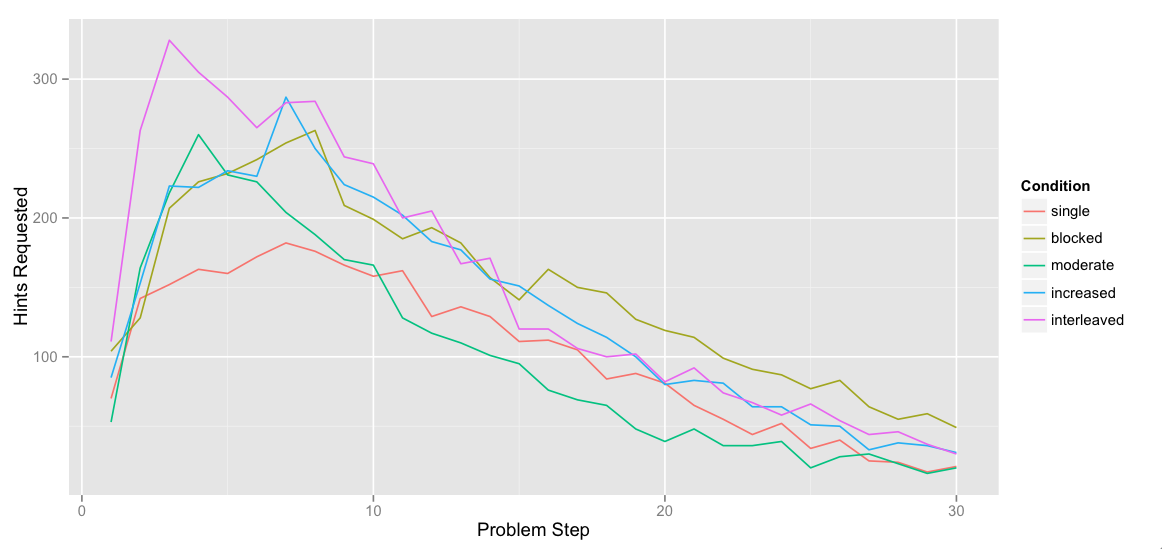
\includegraphics[scale=.35]{hintsByCondition.png}\\
\caption{The $x$-axis represents the $n_{th}$ interaction with the tutor across all problems. The $y$-axis is the total number of hints requested at the $n_{th}$ step.  }
\label{fig:condition-graph}
\end{figure*}

Note that students who received only one representation start out requesting the fewest hints, but students in the moderate condition eventually need fewer. Such considerations motivated our interest in the temporal distribution of hint behavior at the student level. We fit geometric distributions to the number of steps taken before the first hint request (\emph{firstHintGeom}) and to the number of errors before the first hint (\emph{stubbornGeom}). The estimated parameter is used to characterize the student's hint-seeking propensity in general and hint-seeking propensity when faced with adversity. For example, students in the first quintile of \emph{stubbornGeom} seek help soon after making a mistake, whereas students in the fifth quintile don't change their hint-seeking behavior even after making a large number of errors. Students in the first quintile of \emph{firstHintGeom} are likely to request hints early in a problem, whereas students in the fifth quintile are unlikely to request hints at any point.
\begin{table*}[htbp]
\caption{Summary Statistics for Variables Used in Clustering}
\begin{center}
\begin{tabular}{| l || c | c || c | c | c || c | c | c | c | c |}
\hline
&mean& sd&median&min&max&20\%&40\%&60\%&	80\%&100\%\\ \hline \hline
\textbf{hints\_req}&0.78&1.27&0.34&0&11.22&0.06&0.19&0.5&1.31&11.22\\ \hline
\textbf{num\_errors}&2.21&1.27&1.92&0.34&8.39&1.15&1.7&2.18&3.19&8.39\\ \hline 
\textbf{firstHintGeom}&0.35&0.27&0.27&0.04&1&0.13&0.2&0.33&0.57&1\\ \hline
\textbf{stubbornGeom}&0.36&0.21&0.31&0.07&1&0.19&0.27&0.38&0.47&1\\ \hline
\textbf{NumBOH}&0.04&0.08&0&0&0.62&0&0&0.01&0.05&0.63\\ \hline
 \end{tabular}
\end{center}
\label{tab:sumstats}
\end{table*}




\subsection{Latent Class Analysis}
\label{sec:LCA}

Latent Class Analysis (LCA) is a modeling technique that determines subtypes based on multinomial distributions. We use LCA to categorize students into \emph{latent classes} using discretized versions of the features described above. Table \ref{tab:sumstats} shows summary statistics and cut-off points for the extracted features. The model maps a set of observed categorical variables onto a set of inferred latent variables. 

We note that the categorical nature of the model has the potential to add some noise, since we must select numeric cutoffs to transform our variables into nominals. However, categorical models can offer greater interpretability by allowing us to organize our data into a small set of variables, which forms the basis for categorizing students into a small set of meaningful homogenous groups. Furthermore, it is not unreasonable to suspect that our variables are in some sense ``truly'' categorical. 

The formal representation of LCA begins with $j = 1 \ldots J$ observed variables, where each such variable $j$ has a set of response variables $r_{j} = 1,\ldots,R_{j}$. Each student has a distinct response pattern $y = (r_{1},\ldots,r_{j})$.

Now we need to consider the latent classes. Let $L$ be a latent variable with latent classes $c~=~1,\ldots,C$. Furthermore, let $\gamma_{c}$ be the probability of membership in class $c$. Note that latent classes are exhaustive and mutually exclusive, so each student is a member of exactly one latent class. We also need to define the item-response probability $\rho_{j,r_{j}|c}$, which is the probability of response $r_{j}$ to observed variable $j$, conditional on membership in latent class $c$. Each student provides exactly one response alternative to variable $j$. Given these constraints, note that
\[ \sum_{c=1}^{C} \gamma_{c} = 1,\quad \sum_{r_{j}=1}^{R_{j}} \rho_{j,r_{j}|c} = 1. \] 

Now that we have defined key variables, we can define the probability of observing a particular response vector based on the $\gamma$'s and $\rho$'s:
\begin{align}
P(Y = y) = \sum_{c=1}^{C} \gamma_{c} \prod_{j=1}^{J} \prod_{r_{j}=1}^{R_{j}} \rho_{j,r_{j}|c}^{I(y_{j} = r_{j})}
\label{eqn:LCA-final}
\end{align}
where the indicator function $I(y_{j} = r_{j})$ equals 1 when the response variable $j = r_{j}$. The parameters $\gamma_{c}$ and $\rho_{j,r_{j}|c}$ are estimated by EM. Since EM is sensitive to starting probabilities, we pick the maximum likelihood over twenty-five runs. LCA is very similar to other EM-based algorithms. In fact, LCA is an application of multivariate mixture estimation using categorical variables with an additional local independence assumption, meaning that the observed variables are independent of each other conditional on the latent variable. This is a simplifying assumption similar to the one made in Naive Bayes; without it Equation \ref{eqn:LCA-final} would have to be much more complicated. There is some work on relaxing this independence assumption \cite{Hagenaars1988}. To run latent class analysis, we used \texttt{poLCA}, a freely available R package\footnote{\url{http://userwww.service.emory.edu/~dlinzer/poLCA/}}.


Note that unlike some common clustering algorithms (e.g., k-means), LCA produces ``fuzzy'' clusters--probability distributions over features for each class. To cluster students we  identify their most likely class:
\begin{align}
\argmax_{c} P(Y = y \;|\; L = c) = \argmax_{c} \gamma_{c} \prod_{j=1}^{J} \prod_{r_{j}=1}^{R_{j}} \rho_{j,r_{j}|c}^{I(y_{j} = r_{j})}
\label{eqn:LCA-argmax}
\end{align}

We still need to fix $C$, the number of latent classes. We use two complexity-penalized log-likelihood scores to select an appropriate $C$: Akaike information criterion (AIC) and Bayesian information criterion (BIC). Plotting these statistics as we increment the number of latent classes, we look for a ``knee'' where both statistics either bottom-out or level off to identify the optimal value of $C$.

\section{Results}
\label{sec:results}

Figure \ref{fig:lca-test-statistics} shows the parameter selection process described in section 4.2. Note that we chose to model four latent classes because BIC bottoms out and AIC levels off at that point.

\begin{figure}[htbp]
%\centering
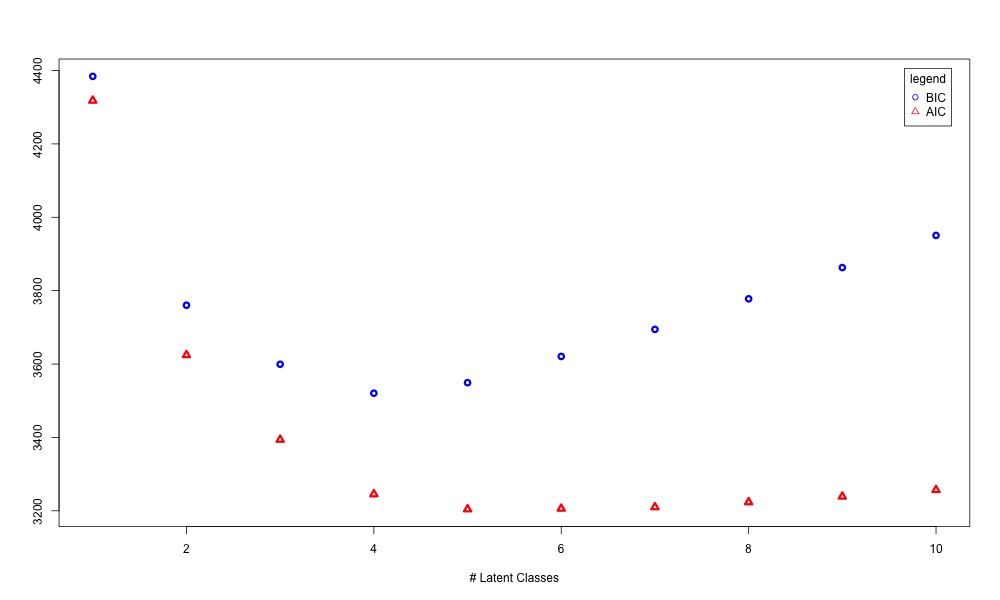
\includegraphics[scale=0.25]{lca-stats-plot.png}
\caption{AIC and BIC over increasing number of latent classes. BIC bottoms out and AIC levels off at four classes, so we conclude that four latent classes best fits the data.}
\label{fig:lca-test-statistics}
\end{figure}
\subsection{Exploring the Latent Classes}

After selecting the appropriate $C$ parameter, we extract membership probabilities for the individual students. Given a latent class, we know the probability distribution over each feature, and use Equation \ref{eqn:LCA-argmax} to identify the most likely class for each student.

The feature distributions over each class are represented graphically in Figure \ref{fig:lca-class-viz}. Note that each feature is listed along the horizontal $x$-axis, the value each variable takes takes is along the front-to-back $y$-axis, and the probability that the feature takes that value is given along the vertical $z$-axis. For example, consider the \emph{hints\_req} feature (average hints requested per problem) in Class 2. In that class, with high probability, students requested many hints (i.e., the highest categorical value for hints) per problem on average. As another example, students in Class 1 are more likely to make a moderate number of errors, though other error levels also occur with nontrivial probabilities. Note that lower values of \emph{firstHintGeom} and \emph{stubbornGeom} indicate a steep geometric slope, corresponding to a higher hint-seeking propensity.

How do we interpret latent class membership? Students in Class 1 are ``Moderate'', they ask for a moderate number of hints, make a moderate number of errors, and are moderately responsive to the interface. Students in Class 2 are ``Interactive'', they make a lot of errors, but respond by requesting many hints. These students are proactive in asking for help and are not shy about using the resources the cognitive tutor makes available. Students in Class 3 are ``Confident'', they don't ask for hints, but they don't seem to need them. Finally, the students in Class 4 are ``Stubborn'', they are fairly mixed in error-profile but they don't respond to mistakes with hint-requests. These students are not using all the resources that the cognitive tutor makes available.

\begin{figure*}[htbp]
\centering
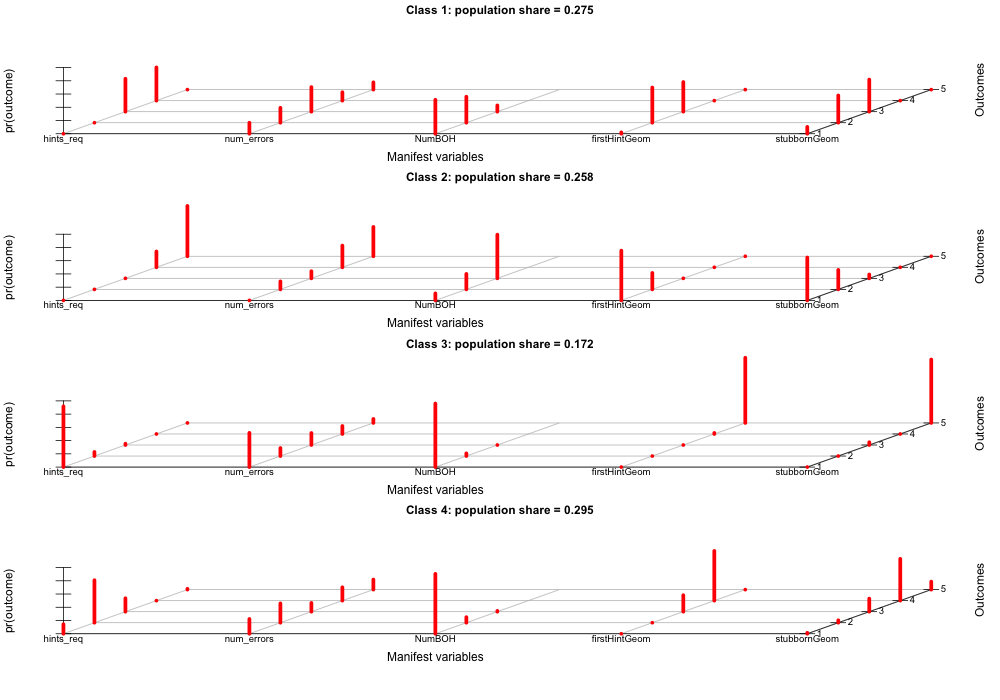
\includegraphics[scale=0.4]{lca-class-viz.png}
\caption{Visualization of feature distributions for each latent class. The left-to-right $x$-axis identifies each feature, the front-to-back $y$-axis identifies which value that feature takes, and the top-to-bottom $z$-axis describes the probability that the feature takes the value. Thus, given a feature and a class, the $z$-axis also describes the probability distribution over that feature in that class.}
\label{fig:lca-class-viz}
\end{figure*}


\subsection{Condition and Outcome} 
We construct a measure of student improvement and knowledge consolidation using the pre-test and the delayed post-test: 
\begin{center}
Adjusted Delayed Post-Test Score = $\frac{\text{post\_test} - \text{pre\_test}}{1-\text{pre\_test}}$
\end{center}
We then construct terciles of the Adjusted Delayed Post-Test Score and run a Chi-squared test for independence of outcome from experimental condition. Confirming previous results, we reject independence at a $p$-value of .024 (See Table 3). 
\subsection{Cluster Membership and Outcome}
We run a Chi-squared test for independence of latent class membership from outcome on the delayed post-test score. We reject independence at a $p$-value of .0075 (See Table 2). The problem-solving behaviors encoded by latent class membership are highly relevant to a student's learning outcome.
\begin{table}[hbtp]
\caption{Latent Class by Tercile of Adjusted Delayed Post-Test Score}
 \begin{center}
\begin{tabular}{|l || c | c | c |}
\hline
&33\%&66\%&99\%\\ \hline \hline
  \emph{LC 1}  &   20& 35& 29 \\ \hline
  \emph{LC 2}&   33& 26& 14 \\ \hline
\emph{LC 3}& 13& 15& 22 \\ \hline
  \emph{LC 4} & 31& 20& 32 \\ \hline
 \end{tabular}
\\$\mathcal{X}^2$ = 17.52, df = 6, p-value = {\bf 0.0075}
\end{center}
\label{default}
\end{table}

\subsection{Condition and Cluster Membership}

We may worry that experimental condition is inducing latent class membership. If this were the case, we would not be detecting pre-existing student profiles, but detecting an artifact of the experimental design. Using the Chi-squared test, we fail to reject independence at a $p$-value of $.38$ (See Table 3). It is therefore likely that our latent classes are detecting genuinely different student profiles, independent of experimental condition. 

\begin{table*}[hbtp]
\caption{Condition by Tercile of Adjusted Delayed Post-Test Score (left) and Latent Class (right).}
 \begin{center}
\begin{tabular}{|l || c | c | c |}
\hline
&33\%&66\%&99\%\\ \hline \hline
  \textbf{blocked}  &   14& 29& 20 \\ \hline
  \textbf{increased}&   22& 20& 20 \\ \hline
\textbf{interleaved}& 13& 21& 18 \\ \hline
  \textbf{moderate} &   18& 13& 22 \\ \hline
    \textbf{single} &      30& 13& 17 \\ \hline
 \end{tabular}
%\end{center}
\label{default}
%\end{table}
\quad
%\begin{table}[hbtp]
%\caption{Experimental Condition and Latent Class}
% \begin{center}
\begin{tabular}{|l || c | c | c | c |}
\hline
&\emph{LC 1}&\emph{LC 2}&\emph{LC 3}&\emph{LC 4}\\ \hline \hline
\textbf{blocked}&     13& 15& 10& 25\\ \hline
\textbf{increased}&   21& 16& 10& 15\\ \hline
\textbf{interleaved}& 17& 18&  7& 10\\ \hline
\textbf{moderate}&    18& 10& 12& 13\\ \hline
\textbf{single}&      15& 14& 11& 20\\ \hline
 \end{tabular}
 \end{center}
\hspace{60pt}$\mathcal{X}^2$ = 17.65, df = 8, p-value = {\bf 0.024} \hspace{30pt}$\mathcal{X}^2$ = 12.85, df = 12, p-value = 0.38
\label{default}
\end{table*}
\begin{table*}[htbp]
\caption{Condition and Tercile of Adjusted Delayed Post-Test Score, by Latent Class  }
 \begin{center}
\begin{tabular}{|l || c | c | c |}
\hline
\emph{LC 1}&33\%&66\%&99\%\\ \hline \hline
  \textbf{blocked}&      2&  8& 3\\ \hline
\textbf{increased}&    4&  9&  8 \\ \hline
  \textbf{interleaved}&  4&  9&  4 \\ \hline
     \textbf{moderate}&     4&  5& 9 \\ \hline
       \textbf{single}&       6&  4&  5 \\ \hline
 \end{tabular}
\label{default}
\begin{tabular}{|l || c | c | c |}
\hline
\emph{LC 2}&33\%&66\%&99\%\\ \hline \hline
  \textbf{blocked}&      7&  6& 2 \\ \hline
\textbf{increased}&    9&  5&  2 \\ \hline
  \textbf{interleaved}&  5&  8&  5 \\ \hline
     \textbf{moderate}&     7&  2& 1 \\ \hline
       \textbf{single}&       5&  5&  4 \\ \hline
 \end{tabular}
\\$\mathcal{X}^2$ = 8.08, df = 8, p-value = 0.43\hspace{15pt}$\mathcal{X}^2$ = 6.95, df = 8, p-value = 0.54\\ \hspace{0pt} \\
\label{default}
\begin{tabular}{|l || c | c | c |}
\hline
\emph{LC 3}&33\%&66\%&99\%\\ \hline \hline
  \textbf{blocked}&      0&  5& 5 \\ \hline
\textbf{increased}&    3&  3&  4 \\ \hline
  \textbf{interleaved}&  2&  2&  3 \\ \hline
     \textbf{moderate}&     3&  4& 5 \\ \hline
       \textbf{single}&       5& 1&  5 \\ \hline
 \end{tabular}
\begin{tabular}{|l || c | c | c |}
\hline
\emph{LC 4}&33\%&66\%&99\%\\ \hline \hline
  \textbf{blocked}&      5&  10& 10 \\ \hline
  \textbf{increased}&    6&  3&  6 \\ \hline
  \textbf{interleaved}&  2&  2&  6 \\ \hline
  \textbf{moderate}&     4&  2& 7 \\ \hline
  \textbf{single}&       14&  3&  3 \\ \hline
 \end{tabular}
\\$\mathcal{X}^2$ = 7.41, df = 8, p-value = 0.49\hspace{15pt}$\mathcal{X}^2$ = 17.4837, df = 8, p-value = {\bf 0.025}
\end{center}
\end{table*}
\subsection{Condition, Outcome and Cluster Membership}
Finally, we ask whether we still detect a dependence of outcome on condition within the latent classes we have defined. Interestingly, we find that latent class membership screens off condition from outcome for all classes but the fourth (See Table 4). Recall that these students rarely requested hints, even when they encountered difficulty. Our results suggest that since these students are not taking full advantage of the other resources the tutor makes available, it is the multiple representation condition that most strongly determines their learning outcome. The problem-solving behaviors of students in the other classes makes them insensitive to experimental condition. 

\subsection{Class Stability}

\begin{figure}
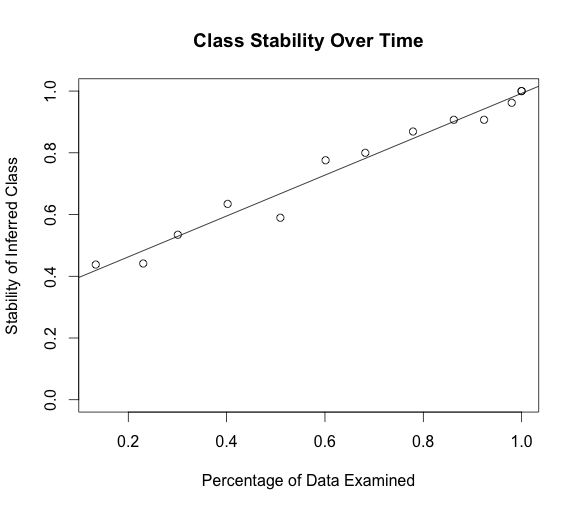
\includegraphics[scale=.6]{class-stability.png}
\caption{TODO}
\label{fig:class-stability}
\end{figure}

See Figure \ref{fig:class-stability}

\section{Conclusion \& Future Work}
\label{sec:conclusion}

We estimated a latent class model to classify students into four groups based on their error-rates and hint-seeking behaviors. We detected dependence of experimental condition and post-test outcome only in the class of students characterized by high-error rate and low hint-seeking propensity. That is, students who did not take full advantage of the resources that the Mathtutor offered were the ones most strongly affected by experimental condition. These students may not have the meta-cognitive skills required to know when to seek hints \cite{Aleven2006}. Our methods could be used by intelligent tutoring systems designers to detect students with this profile in real time. Tutoring systems could then intervene to target these students with multiple representations and to scaffold their hint-seeking behaviors. Future research into  the mediating mechanisms of multiple representations could leverage our results to identify the relevant student sub-populations to investigate. 
\balancecolumns
% That's all folks!

\bibliographystyle{abbrv}
\bibliography{references}

\end{document}
